\documentclass[twoside]{book}

% Packages required by doxygen
\usepackage{fixltx2e}
\usepackage{calc}
\usepackage{doxygen}
\usepackage[export]{adjustbox} % also loads graphicx
\usepackage{graphicx}
\usepackage[utf8]{inputenc}
\usepackage{makeidx}
\usepackage{multicol}
\usepackage{multirow}
\PassOptionsToPackage{warn}{textcomp}
\usepackage{textcomp}
\usepackage[nointegrals]{wasysym}
\usepackage[table]{xcolor}

% NLS support packages
\usepackage[spanish]{babel}
% Font selection
\usepackage[T1]{fontenc}
\usepackage[scaled=.90]{helvet}
\usepackage{courier}
\usepackage{amssymb}
\usepackage{sectsty}
\renewcommand{\familydefault}{\sfdefault}
\allsectionsfont{%
  \fontseries{bc}\selectfont%
  \color{darkgray}%
}
\renewcommand{\DoxyLabelFont}{%
  \fontseries{bc}\selectfont%
  \color{darkgray}%
}
\newcommand{\+}{\discretionary{\mbox{\scriptsize$\hookleftarrow$}}{}{}}

% Page & text layout
\usepackage{geometry}
\geometry{%
  a4paper,%
  top=2.5cm,%
  bottom=2.5cm,%
  left=2.5cm,%
  right=2.5cm%
}
\tolerance=750
\hfuzz=15pt
\hbadness=750
\setlength{\emergencystretch}{15pt}
\setlength{\parindent}{0cm}
\setlength{\parskip}{3ex plus 2ex minus 2ex}
\makeatletter
\renewcommand{\paragraph}{%
  \@startsection{paragraph}{4}{0ex}{-1.0ex}{1.0ex}{%
    \normalfont\normalsize\bfseries\SS@parafont%
  }%
}
\renewcommand{\subparagraph}{%
  \@startsection{subparagraph}{5}{0ex}{-1.0ex}{1.0ex}{%
    \normalfont\normalsize\bfseries\SS@subparafont%
  }%
}
\makeatother

% Headers & footers
\usepackage{fancyhdr}
\pagestyle{fancyplain}
\fancyhead[LE]{\fancyplain{}{\bfseries\thepage}}
\fancyhead[CE]{\fancyplain{}{}}
\fancyhead[RE]{\fancyplain{}{\bfseries\leftmark}}
\fancyhead[LO]{\fancyplain{}{\bfseries\rightmark}}
\fancyhead[CO]{\fancyplain{}{}}
\fancyhead[RO]{\fancyplain{}{\bfseries\thepage}}
\fancyfoot[LE]{\fancyplain{}{}}
\fancyfoot[CE]{\fancyplain{}{}}
\fancyfoot[RE]{\fancyplain{}{\bfseries\scriptsize Generado por Doxygen }}
\fancyfoot[LO]{\fancyplain{}{\bfseries\scriptsize Generado por Doxygen }}
\fancyfoot[CO]{\fancyplain{}{}}
\fancyfoot[RO]{\fancyplain{}{}}
\renewcommand{\footrulewidth}{0.4pt}
\renewcommand{\chaptermark}[1]{%
  \markboth{#1}{}%
}
\renewcommand{\sectionmark}[1]{%
  \markright{\thesection\ #1}%
}

% Indices & bibliography
\usepackage{natbib}
\usepackage[titles]{tocloft}
\setcounter{tocdepth}{3}
\setcounter{secnumdepth}{5}
\makeindex

% Hyperlinks (required, but should be loaded last)
\usepackage{ifpdf}
\ifpdf
  \usepackage[pdftex,pagebackref=true]{hyperref}
\else
  \usepackage[ps2pdf,pagebackref=true]{hyperref}
\fi
\hypersetup{%
  colorlinks=true,%
  linkcolor=blue,%
  citecolor=blue,%
  unicode%
}

% Custom commands
\newcommand{\clearemptydoublepage}{%
  \newpage{\pagestyle{empty}\cleardoublepage}%
}

\usepackage{caption}
\captionsetup{labelsep=space,justification=centering,font={bf},singlelinecheck=off,skip=4pt,position=top}

%===== C O N T E N T S =====

\begin{document}

% Titlepage & ToC
\hypersetup{pageanchor=false,
             bookmarksnumbered=true,
             pdfencoding=unicode
            }
\pagenumbering{roman}
\begin{titlepage}
\vspace*{7cm}
\begin{center}%
{\Large Practica 3 }\\
\vspace*{1cm}
{\large Generado por Doxygen 1.8.11}\\
\end{center}
\end{titlepage}
\clearemptydoublepage
\tableofcontents
\clearemptydoublepage
\pagenumbering{arabic}
\hypersetup{pageanchor=true}

%--- Begin generated contents ---
\chapter{Índice de clases}
\section{Lista de clases}
Lista de las clases, estructuras, uniones e interfaces con una breve descripción\+:\begin{DoxyCompactList}
\item\contentsline{section}{\hyperlink{struct__Apuesta}{\+\_\+\+Apuesta} \\*Estructura apuesta }{\pageref{struct__Apuesta}}{}
\item\contentsline{section}{\hyperlink{struct__Caballo}{\+\_\+\+Caballo} \\*Estructura caballo }{\pageref{struct__Caballo}}{}
\item\contentsline{section}{\hyperlink{struct__Carrera}{\+\_\+\+Carrera} \\*Estructura carrera }{\pageref{struct__Carrera}}{}
\item\contentsline{section}{\hyperlink{struct__Mensaje}{\+\_\+\+Mensaje} \\*Estructura mensaje que contiene todos sus parametros necesarios para la realización del ejercicio con colas de mensajes }{\pageref{struct__Mensaje}}{}
\item\contentsline{section}{\hyperlink{struct__Monitor}{\+\_\+\+Monitor} \\*Estructura monitor }{\pageref{struct__Monitor}}{}
\item\contentsline{section}{\hyperlink{struct__Ventanilla}{\+\_\+\+Ventanilla} \\*Estructura ventanilla }{\pageref{struct__Ventanilla}}{}
\end{DoxyCompactList}

\chapter{Indice de archivos}
\section{Lista de archivos}
Lista de todos los archivos documentados y con descripciones breves\+:\begin{DoxyCompactList}
\item\contentsline{section}{\hyperlink{ejercicio10_8c}{ejercicio10.\+c} \\*Implementa el ejercicio 10 de mascaras }{\pageref{ejercicio10_8c}}{}
\item\contentsline{section}{\hyperlink{ejercicio3a_8c}{ejercicio3a.\+c} \\*Implementa el ejercicio 3a de procesos con un solo padre }{\pageref{ejercicio3a_8c}}{}
\item\contentsline{section}{\hyperlink{ejercicio3b_8c}{ejercicio3b.\+c} \\*Implementa el ejercicio 3b de hilos de un proceso }{\pageref{ejercicio3b_8c}}{}
\item\contentsline{section}{\hyperlink{ejercicio4a_8c}{ejercicio4a.\+c} \\*Implementa el ejercicio 4a de multiplicacion de matrices }{\pageref{ejercicio4a_8c}}{}
\item\contentsline{section}{\hyperlink{ejercicio4b_8c}{ejercicio4b.\+c} \\*Implementa el ejercicio 4b de multiplicacion de matrices }{\pageref{ejercicio4b_8c}}{}
\item\contentsline{section}{\hyperlink{ejercicio6_8c}{ejercicio6.\+c} \\*Implementa el ejercicio 6 de señales }{\pageref{ejercicio6_8c}}{}
\end{DoxyCompactList}

\chapter{Documentación de las clases}
\hypertarget{structinfo}{}\section{Referencia de la Estructura info}
\label{structinfo}\index{info@{info}}


Estructura info que contiene los parametros pedidos para la reserva de un bloque de memoria.  


\subsection*{Atributos públicos}
\begin{DoxyCompactItemize}
\item 
char \hyperlink{structinfo_aaa02777b492865c2877852cb159803b1}{nombre} \mbox{[}80\mbox{]}
\item 
int \hyperlink{structinfo_afe86f23d8bd5fd8d139e39a5b1a01171}{id}
\end{DoxyCompactItemize}


\subsection{Descripción detallada}
Estructura info que contiene los parametros pedidos para la reserva de un bloque de memoria. 

\subsection{Documentación de los datos miembro}
\index{info@{info}!id@{id}}
\index{id@{id}!info@{info}}
\subsubsection[{\texorpdfstring{id}{id}}]{\setlength{\rightskip}{0pt plus 5cm}int info\+::id}\hypertarget{structinfo_afe86f23d8bd5fd8d139e39a5b1a01171}{}\label{structinfo_afe86f23d8bd5fd8d139e39a5b1a01171}
Identificador \index{info@{info}!nombre@{nombre}}
\index{nombre@{nombre}!info@{info}}
\subsubsection[{\texorpdfstring{nombre}{nombre}}]{\setlength{\rightskip}{0pt plus 5cm}char info\+::nombre\mbox{[}80\mbox{]}}\hypertarget{structinfo_aaa02777b492865c2877852cb159803b1}{}\label{structinfo_aaa02777b492865c2877852cb159803b1}
Nombre del usuario 

La documentación para esta estructura fue generada a partir del siguiente fichero\+:\begin{DoxyCompactItemize}
\item 
\hyperlink{ejercicio2_8c}{ejercicio2.\+c}\end{DoxyCompactItemize}

\chapter{Documentación de archivos}
\hypertarget{ejercicio2_8c}{}\section{Referencia del Archivo ejercicio2.\+c}
\label{ejercicio2_8c}\index{ejercicio2.\+c@{ejercicio2.\+c}}


Implementa el ejercicio 2 de memoria compartida.  


{\ttfamily \#include $<$stdio.\+h$>$}\\*
{\ttfamily \#include $<$stdlib.\+h$>$}\\*
{\ttfamily \#include $<$sys/shm.\+h$>$}\\*
{\ttfamily \#include $<$sys/types.\+h$>$}\\*
{\ttfamily \#include $<$sys/ipc.\+h$>$}\\*
{\ttfamily \#include $<$signal.\+h$>$}\\*
{\ttfamily \#include $<$unistd.\+h$>$}\\*
Dependencia gráfica adjunta para ejercicio2.\+c\+:
\nopagebreak
\begin{figure}[H]
\begin{center}
\leavevmode
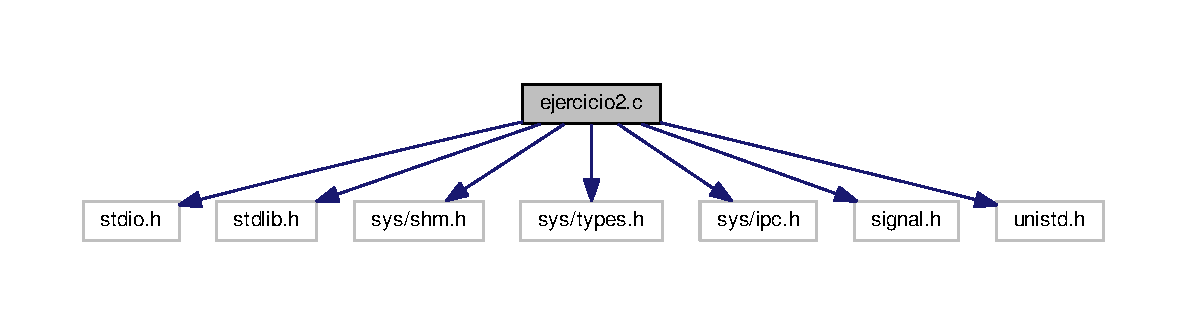
\includegraphics[width=350pt]{ejercicio2_8c__incl}
\end{center}
\end{figure}
\subsection*{Clases}
\begin{DoxyCompactItemize}
\item 
struct \hyperlink{structinfo}{info}
\begin{DoxyCompactList}\small\item\em Estructura info que contiene los parametros pedidos para la reserva de un bloque de memoria. \end{DoxyCompactList}\end{DoxyCompactItemize}
\subsection*{\textquotesingle{}defines\textquotesingle{}}
\begin{DoxyCompactItemize}
\item 
\#define \hyperlink{ejercicio2_8c_a8ae9d53f33f46cfcfcb9736e6351452a}{K\+EY}~1300\hypertarget{ejercicio2_8c_a8ae9d53f33f46cfcfcb9736e6351452a}{}\label{ejercicio2_8c_a8ae9d53f33f46cfcfcb9736e6351452a}

\begin{DoxyCompactList}\small\item\em Definicion de la clave. \end{DoxyCompactList}\item 
\#define \hyperlink{ejercicio2_8c_a68c15c5fb7f7c6f707903e6a46ab0557}{F\+I\+L\+E\+K\+EY}~\char`\"{}/bin/cat\char`\"{}\hypertarget{ejercicio2_8c_a68c15c5fb7f7c6f707903e6a46ab0557}{}\label{ejercicio2_8c_a68c15c5fb7f7c6f707903e6a46ab0557}

\begin{DoxyCompactList}\small\item\em Definicion de la clave de fichero. \end{DoxyCompactList}\end{DoxyCompactItemize}
\subsection*{\textquotesingle{}typedefs\textquotesingle{}}
\begin{DoxyCompactItemize}
\item 
typedef struct \hyperlink{structinfo}{info} \hyperlink{ejercicio2_8c_a163511f3dadd6f89b69b2c2b6d40dcf7}{Info}\hypertarget{ejercicio2_8c_a163511f3dadd6f89b69b2c2b6d40dcf7}{}\label{ejercicio2_8c_a163511f3dadd6f89b69b2c2b6d40dcf7}

\begin{DoxyCompactList}\small\item\em Estructura info que contiene los parametros pedidos para la reserva de un bloque de memoria. \end{DoxyCompactList}\end{DoxyCompactItemize}
\subsection*{Funciones}
\begin{DoxyCompactItemize}
\item 
void \hyperlink{ejercicio2_8c_a0ea23ff7004eb4a35a58394731fc9474}{capturar} (int signal)
\begin{DoxyCompactList}\small\item\em funcion de captura de señales \end{DoxyCompactList}\item 
int \hyperlink{ejercicio2_8c_a0ddf1224851353fc92bfbff6f499fa97}{main} (int argc, char $\ast$argv\mbox{[}$\,$\mbox{]})
\begin{DoxyCompactList}\small\item\em funcion principal que genera nhijos y que implementa todo lo que debe realizar tanto el padre como sus hijos \end{DoxyCompactList}\end{DoxyCompactItemize}
\subsection*{Variables}
\begin{DoxyCompactItemize}
\item 
\hyperlink{ejercicio2_8c_a163511f3dadd6f89b69b2c2b6d40dcf7}{Info} $\ast$ \hyperlink{ejercicio2_8c_a1a7947f4bb22d269cbbdca314e89c2af}{datos} = N\+U\+LL
\end{DoxyCompactItemize}


\subsection{Descripción detallada}
Implementa el ejercicio 2 de memoria compartida. 

\begin{DoxyAuthor}{Autor}
Andres Salas \href{mailto:andres.salas@estudiante.uam.es}{\tt andres.\+salas@estudiante.\+uam.\+es} 

Antonio Martin \href{mailto:antonio.martinmasuda@estudiante.uam.es}{\tt antonio.\+martinmasuda@estudiante.\+uam.\+es} 
\end{DoxyAuthor}
\begin{DoxyNote}{Nota}
Grupo 2202 
\end{DoxyNote}
\begin{DoxyVersion}{Versión}
1.\+0 
\end{DoxyVersion}
\begin{DoxyDate}{Fecha}
24/03/2017 
\end{DoxyDate}


\subsection{Documentación de las funciones}
\index{ejercicio2.\+c@{ejercicio2.\+c}!capturar@{capturar}}
\index{capturar@{capturar}!ejercicio2.\+c@{ejercicio2.\+c}}
\subsubsection[{\texorpdfstring{capturar(int signal)}{capturar(int signal)}}]{\setlength{\rightskip}{0pt plus 5cm}void capturar (
\begin{DoxyParamCaption}
\item[{int}]{signal}
\end{DoxyParamCaption}
)}\hypertarget{ejercicio2_8c_a0ea23ff7004eb4a35a58394731fc9474}{}\label{ejercicio2_8c_a0ea23ff7004eb4a35a58394731fc9474}


funcion de captura de señales 


\begin{DoxyParams}{Parámetros}
{\em signal} & señal pasada \\
\hline
\end{DoxyParams}
\index{ejercicio2.\+c@{ejercicio2.\+c}!main@{main}}
\index{main@{main}!ejercicio2.\+c@{ejercicio2.\+c}}
\subsubsection[{\texorpdfstring{main(int argc, char $\ast$argv[])}{main(int argc, char *argv[])}}]{\setlength{\rightskip}{0pt plus 5cm}int main (
\begin{DoxyParamCaption}
\item[{int}]{argc, }
\item[{char $\ast$}]{argv\mbox{[}$\,$\mbox{]}}
\end{DoxyParamCaption}
)}\hypertarget{ejercicio2_8c_a0ddf1224851353fc92bfbff6f499fa97}{}\label{ejercicio2_8c_a0ddf1224851353fc92bfbff6f499fa97}


funcion principal que genera nhijos y que implementa todo lo que debe realizar tanto el padre como sus hijos 


\begin{DoxyParams}{Parámetros}
{\em argc} & contiene el número de parámetros totales pasados \\
\hline
{\em argv} & contiene los parámetros pasados por el usuario \\
\hline
\end{DoxyParams}
\begin{DoxyReturn}{Devuelve}
int\+: valor de exito (OK) o fracaso (E\+R\+R\+OR) 
\end{DoxyReturn}


\subsection{Documentación de las variables}
\index{ejercicio2.\+c@{ejercicio2.\+c}!datos@{datos}}
\index{datos@{datos}!ejercicio2.\+c@{ejercicio2.\+c}}
\subsubsection[{\texorpdfstring{datos}{datos}}]{\setlength{\rightskip}{0pt plus 5cm}{\bf Info}$\ast$ datos = N\+U\+LL}\hypertarget{ejercicio2_8c_a1a7947f4bb22d269cbbdca314e89c2af}{}\label{ejercicio2_8c_a1a7947f4bb22d269cbbdca314e89c2af}
Inicializacion de la estructura a N\+U\+LL 
\hypertarget{ejercicio5_8c}{}\section{Referencia del Archivo ejercicio5.\+c}
\label{ejercicio5_8c}\index{ejercicio5.\+c@{ejercicio5.\+c}}


Implementa el ejercicio 5 de semaforos (test con B\+I\+N\+A\+R\+I\+OS)  


{\ttfamily \#include \char`\"{}semaforos.\+h\char`\"{}}\\*
{\ttfamily \#include $<$sys/sem.\+h$>$}\\*
Dependencia gráfica adjunta para ejercicio5.\+c\+:\nopagebreak
\begin{figure}[H]
\begin{center}
\leavevmode
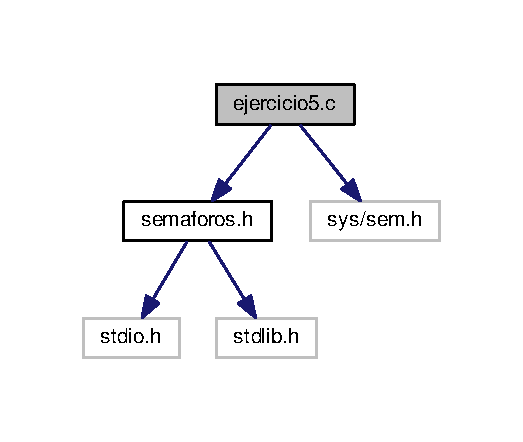
\includegraphics[width=251pt]{ejercicio5_8c__incl}
\end{center}
\end{figure}
\subsection*{\textquotesingle{}defines\textquotesingle{}}
\begin{DoxyCompactItemize}
\item 
\#define \hyperlink{ejercicio5_8c_ada831b9e37399bf906c8184a888e28cd}{S\+E\+M\+K\+EY}~75798\hypertarget{ejercicio5_8c_ada831b9e37399bf906c8184a888e28cd}{}\label{ejercicio5_8c_ada831b9e37399bf906c8184a888e28cd}

\begin{DoxyCompactList}\small\item\em Define la clave precompartida de los semaforos. \end{DoxyCompactList}\item 
\#define \hyperlink{ejercicio5_8c_a95c81905ff3d55e62fb763f407f9fab1}{N\+\_\+\+S\+E\+M\+A\+F\+O\+R\+OS}~3\hypertarget{ejercicio5_8c_a95c81905ff3d55e62fb763f407f9fab1}{}\label{ejercicio5_8c_a95c81905ff3d55e62fb763f407f9fab1}

\begin{DoxyCompactList}\small\item\em Define el numero total de semaforos. \end{DoxyCompactList}\end{DoxyCompactItemize}
\subsection*{Funciones}
\begin{DoxyCompactItemize}
\item 
int \hyperlink{ejercicio5_8c_ae66f6b31b5ad750f1fe042a706a4e3d4}{main} ()
\begin{DoxyCompactList}\small\item\em funcion principal/ test con semaforos B\+I\+N\+A\+R\+I\+OS siguiendo el codigo se explica que se va realizando \end{DoxyCompactList}\end{DoxyCompactItemize}


\subsection{Descripción detallada}
Implementa el ejercicio 5 de semaforos (test con B\+I\+N\+A\+R\+I\+OS) 

\begin{DoxyAuthor}{Autor}
Andres Salas \href{mailto:andres.salas@estudiante.uam.es}{\tt andres.\+salas@estudiante.\+uam.\+es} 

Antonio Martin \href{mailto:antonio.martinmasuda@estudiante.uam.es}{\tt antonio.\+martinmasuda@estudiante.\+uam.\+es} 
\end{DoxyAuthor}
\begin{DoxyNote}{Nota}
Grupo 2202 
\end{DoxyNote}
\begin{DoxyVersion}{Versión}
1.\+0 
\end{DoxyVersion}
\begin{DoxyDate}{Fecha}
31/03/2017 
\end{DoxyDate}


\subsection{Documentación de las funciones}
\index{ejercicio5.\+c@{ejercicio5.\+c}!main@{main}}
\index{main@{main}!ejercicio5.\+c@{ejercicio5.\+c}}
\subsubsection[{\texorpdfstring{main()}{main()}}]{\setlength{\rightskip}{0pt plus 5cm}int main (
\begin{DoxyParamCaption}
{}
\end{DoxyParamCaption}
)}\hypertarget{ejercicio5_8c_ae66f6b31b5ad750f1fe042a706a4e3d4}{}\label{ejercicio5_8c_ae66f6b31b5ad750f1fe042a706a4e3d4}


funcion principal/ test con semaforos B\+I\+N\+A\+R\+I\+OS siguiendo el codigo se explica que se va realizando 

\begin{DoxyReturn}{Devuelve}
int\+: valor de exito (OK) o fracaso (E\+R\+R\+OR) 
\end{DoxyReturn}

\hypertarget{ejercicio5b_8c}{}\section{Referencia del Archivo ejercicio5b.\+c}
\label{ejercicio5b_8c}\index{ejercicio5b.\+c@{ejercicio5b.\+c}}


Implementa el ejercicio 5b de semaforos (test con N-\/\+A\+R\+I\+OS)  


{\ttfamily \#include \char`\"{}semaforos.\+h\char`\"{}}\\*
{\ttfamily \#include $<$sys/sem.\+h$>$}\\*
Dependencia gráfica adjunta para ejercicio5b.\+c\+:\nopagebreak
\begin{figure}[H]
\begin{center}
\leavevmode
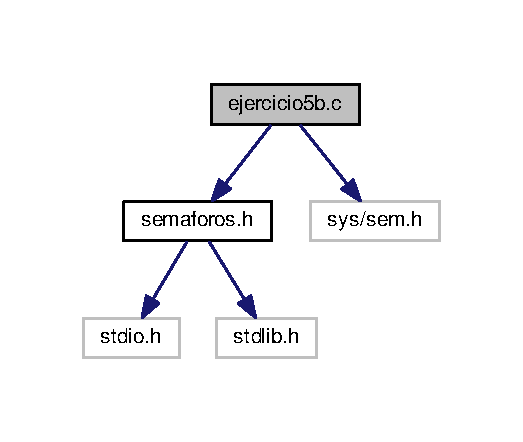
\includegraphics[width=251pt]{ejercicio5b_8c__incl}
\end{center}
\end{figure}
\subsection*{\textquotesingle{}defines\textquotesingle{}}
\begin{DoxyCompactItemize}
\item 
\#define \hyperlink{ejercicio5b_8c_ada831b9e37399bf906c8184a888e28cd}{S\+E\+M\+K\+EY}~75798\hypertarget{ejercicio5b_8c_ada831b9e37399bf906c8184a888e28cd}{}\label{ejercicio5b_8c_ada831b9e37399bf906c8184a888e28cd}

\begin{DoxyCompactList}\small\item\em Define la clave precompartida de los semaforos. \end{DoxyCompactList}\item 
\#define \hyperlink{ejercicio5b_8c_a95c81905ff3d55e62fb763f407f9fab1}{N\+\_\+\+S\+E\+M\+A\+F\+O\+R\+OS}~3\hypertarget{ejercicio5b_8c_a95c81905ff3d55e62fb763f407f9fab1}{}\label{ejercicio5b_8c_a95c81905ff3d55e62fb763f407f9fab1}

\begin{DoxyCompactList}\small\item\em Define el numero total de semaforos. \end{DoxyCompactList}\end{DoxyCompactItemize}
\subsection*{Funciones}
\begin{DoxyCompactItemize}
\item 
int \hyperlink{ejercicio5b_8c_ae66f6b31b5ad750f1fe042a706a4e3d4}{main} ()
\begin{DoxyCompactList}\small\item\em funcion principal/ test con semaforos B\+I\+N\+A\+R\+I\+OS y N-\/\+A\+R\+I\+OS siguiendo el codigo se explica que se va realizando \end{DoxyCompactList}\end{DoxyCompactItemize}


\subsection{Descripción detallada}
Implementa el ejercicio 5b de semaforos (test con N-\/\+A\+R\+I\+OS) 

\begin{DoxyAuthor}{Autor}
Andres Salas \href{mailto:andres.salas@estudiante.uam.es}{\tt andres.\+salas@estudiante.\+uam.\+es} 

Antonio Martin \href{mailto:antonio.martinmasuda@estudiante.uam.es}{\tt antonio.\+martinmasuda@estudiante.\+uam.\+es} 
\end{DoxyAuthor}
\begin{DoxyNote}{Nota}
Grupo 2202 
\end{DoxyNote}
\begin{DoxyVersion}{Versión}
1.\+0 
\end{DoxyVersion}
\begin{DoxyDate}{Fecha}
05/03/2017 
\end{DoxyDate}


\subsection{Documentación de las funciones}
\index{ejercicio5b.\+c@{ejercicio5b.\+c}!main@{main}}
\index{main@{main}!ejercicio5b.\+c@{ejercicio5b.\+c}}
\subsubsection[{\texorpdfstring{main()}{main()}}]{\setlength{\rightskip}{0pt plus 5cm}int main (
\begin{DoxyParamCaption}
{}
\end{DoxyParamCaption}
)}\hypertarget{ejercicio5b_8c_ae66f6b31b5ad750f1fe042a706a4e3d4}{}\label{ejercicio5b_8c_ae66f6b31b5ad750f1fe042a706a4e3d4}


funcion principal/ test con semaforos B\+I\+N\+A\+R\+I\+OS y N-\/\+A\+R\+I\+OS siguiendo el codigo se explica que se va realizando 

\begin{DoxyReturn}{Devuelve}
int\+: valor de exito (OK) o fracaso (E\+R\+R\+OR) 
\end{DoxyReturn}

\hypertarget{ejercicio6_8c}{}\section{Referencia del Archivo ejercicio6.\+c}
\label{ejercicio6_8c}\index{ejercicio6.\+c@{ejercicio6.\+c}}


Implementa el ejercicio 6 de relacion entre procesos padre/hijo.  


{\ttfamily \#include $<$stdio.\+h$>$}\\*
{\ttfamily \#include $<$stdlib.\+h$>$}\\*
{\ttfamily \#include $<$sys/types.\+h$>$}\\*
{\ttfamily \#include $<$sys/wait.\+h$>$}\\*
{\ttfamily \#include $<$unistd.\+h$>$}\\*
Dependencia gráfica adjunta para ejercicio6.\+c\+:\nopagebreak
\begin{figure}[H]
\begin{center}
\leavevmode
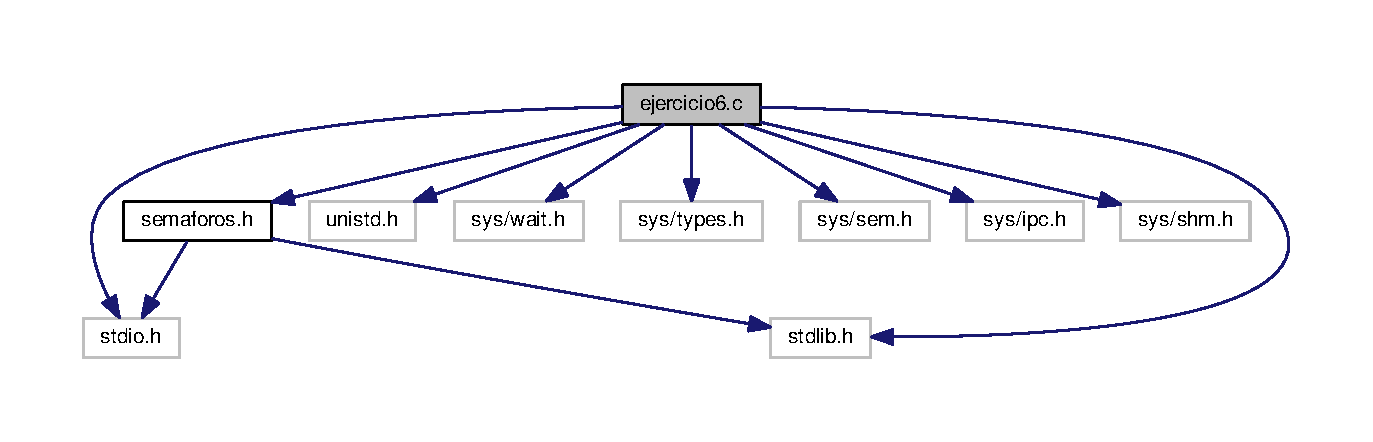
\includegraphics[width=350pt]{ejercicio6_8c__incl}
\end{center}
\end{figure}
\subsection*{\textquotesingle{}defines\textquotesingle{}}
\begin{DoxyCompactItemize}
\item 
\#define \hyperlink{ejercicio6_8c_a4cc8fa399feaab01926e82767a97a96b}{C\+A\+D\+E\+NA}~80
\end{DoxyCompactItemize}
\subsection*{Funciones}
\begin{DoxyCompactItemize}
\item 
int \hyperlink{ejercicio6_8c_a840291bc02cba5474a4cb46a9b9566fe}{main} (void)
\begin{DoxyCompactList}\small\item\em funcion en la que el proceso padre reserva memoria y en el proceso hijo el usuario introduce un nombre \end{DoxyCompactList}\end{DoxyCompactItemize}


\subsection{Descripción detallada}
Implementa el ejercicio 6 de relacion entre procesos padre/hijo. 

\begin{DoxyAuthor}{Autor}
Andres Salas \href{mailto:andres.salas@estudiante.uam.es}{\tt andres.\+salas@estudiante.\+uam.\+es} 

Antonio Martin \href{mailto:antonio.martinmasuda@estudiante.uam.es}{\tt antonio.\+martinmasuda@estudiante.\+uam.\+es} 
\end{DoxyAuthor}
\begin{DoxyNote}{Nota}
Grupo 2202 
\end{DoxyNote}
\begin{DoxyVersion}{Versión}
1.\+0 
\end{DoxyVersion}
\begin{DoxyDate}{Fecha}
10/02/2017 
\end{DoxyDate}


\subsection{Documentación de los \textquotesingle{}defines\textquotesingle{}}
\index{ejercicio6.\+c@{ejercicio6.\+c}!C\+A\+D\+E\+NA@{C\+A\+D\+E\+NA}}
\index{C\+A\+D\+E\+NA@{C\+A\+D\+E\+NA}!ejercicio6.\+c@{ejercicio6.\+c}}
\subsubsection[{\texorpdfstring{C\+A\+D\+E\+NA}{CADENA}}]{\setlength{\rightskip}{0pt plus 5cm}\#define C\+A\+D\+E\+NA~80}\hypertarget{ejercicio6_8c_a4cc8fa399feaab01926e82767a97a96b}{}\label{ejercicio6_8c_a4cc8fa399feaab01926e82767a97a96b}
Numero de caracteres de la cadena 

\subsection{Documentación de las funciones}
\index{ejercicio6.\+c@{ejercicio6.\+c}!main@{main}}
\index{main@{main}!ejercicio6.\+c@{ejercicio6.\+c}}
\subsubsection[{\texorpdfstring{main(void)}{main(void)}}]{\setlength{\rightskip}{0pt plus 5cm}int main (
\begin{DoxyParamCaption}
\item[{void}]{}
\end{DoxyParamCaption}
)}\hypertarget{ejercicio6_8c_a840291bc02cba5474a4cb46a9b9566fe}{}\label{ejercicio6_8c_a840291bc02cba5474a4cb46a9b9566fe}


funcion en la que el proceso padre reserva memoria y en el proceso hijo el usuario introduce un nombre 

\begin{DoxyReturn}{Devuelve}
int\+: valor de exito o fracaso 
\end{DoxyReturn}

\hypertarget{semaforos_8c}{}\section{Referencia del Archivo semaforos.\+c}
\label{semaforos_8c}\index{semaforos.\+c@{semaforos.\+c}}


Implementa el ejercicio 4 de la biblioteca de semaforos.  


{\ttfamily \#include $<$stdio.\+h$>$}\\*
{\ttfamily \#include $<$stdlib.\+h$>$}\\*
{\ttfamily \#include $<$sys/types.\+h$>$}\\*
{\ttfamily \#include $<$sys/ipc.\+h$>$}\\*
{\ttfamily \#include $<$sys/sem.\+h$>$}\\*
{\ttfamily \#include $<$sys/shm.\+h$>$}\\*
{\ttfamily \#include $<$errno.\+h$>$}\\*
{\ttfamily \#include \char`\"{}semaforos.\+h\char`\"{}}\\*
Dependencia gráfica adjunta para semaforos.\+c\+:\nopagebreak
\begin{figure}[H]
\begin{center}
\leavevmode
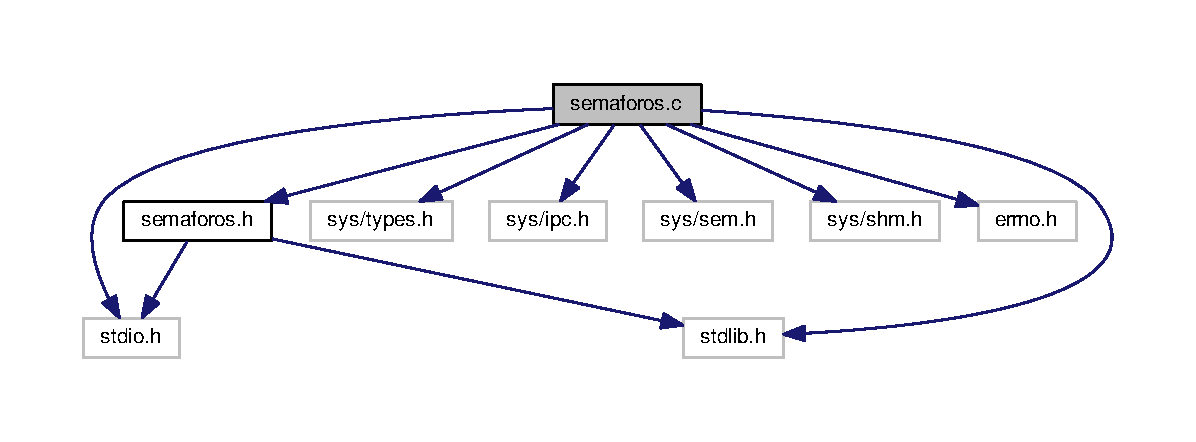
\includegraphics[width=350pt]{semaforos_8c__incl}
\end{center}
\end{figure}
\subsection*{Funciones}
\begin{DoxyCompactItemize}
\item 
int \hyperlink{semaforos_8c_a4af104b0ed37e6ae0289a1059bc6e990}{Inicializar\+\_\+\+Semaforo} (int semid, unsigned short $\ast$array)
\begin{DoxyCompactList}\small\item\em Inicializa los semaforos indicados. \end{DoxyCompactList}\item 
int \hyperlink{semaforos_8c_a731339337960a681efa435a10f12c312}{Borrar\+\_\+\+Semaforo} (int semid)
\begin{DoxyCompactList}\small\item\em Borra un semaforo. \end{DoxyCompactList}\item 
int \hyperlink{semaforos_8c_a16b16dd895b5f4cbe48f1ac8977e8b35}{Crear\+\_\+\+Semaforo} (key\+\_\+t key, int size, int $\ast$semid)
\begin{DoxyCompactList}\small\item\em Crea un semaforo con la clave y el tamaño especificado. Lo inicializa a 0. \end{DoxyCompactList}\item 
int \hyperlink{semaforos_8c_a09cfe06b86766d42e1187644784afb9b}{Down\+\_\+\+Semaforo} (int semid, int num\+\_\+sem, int undo)
\begin{DoxyCompactList}\small\item\em Baja el semaforo indicado. \end{DoxyCompactList}\item 
int \hyperlink{semaforos_8c_ad15a11016ff8903f5907773717c7d479}{Down\+Multiple\+\_\+\+Semaforo} (int semid, int size, int undo, int $\ast$active)
\begin{DoxyCompactList}\small\item\em Baja todos los semaforos del array indicado por active. \end{DoxyCompactList}\item 
int \hyperlink{semaforos_8c_ad282ab72294b1389eeac632ebcddd7dc}{Up\+\_\+\+Semaforo} (int semid, int num\+\_\+sem, int undo)
\begin{DoxyCompactList}\small\item\em Sube el semaforo indicado. \end{DoxyCompactList}\item 
int \hyperlink{semaforos_8c_a56b7305d77fab42b0328171a9603a7f7}{Up\+Multiple\+\_\+\+Semaforo} (int semid, int size, int undo, int $\ast$active)
\begin{DoxyCompactList}\small\item\em Sube todos los semaforos del array indicado por active. \end{DoxyCompactList}\end{DoxyCompactItemize}


\subsection{Descripción detallada}
Implementa el ejercicio 4 de la biblioteca de semaforos. 

\begin{DoxyAuthor}{Autor}
Andres Salas \href{mailto:andres.salas@estudiante.uam.es}{\tt andres.\+salas@estudiante.\+uam.\+es} 

Antonio Martin \href{mailto:antonio.martinmasuda@estudiante.uam.es}{\tt antonio.\+martinmasuda@estudiante.\+uam.\+es} 
\end{DoxyAuthor}
\begin{DoxyNote}{Nota}
Grupo 2202 
\end{DoxyNote}
\begin{DoxyVersion}{Versión}
1.\+0 
\end{DoxyVersion}
\begin{DoxyDate}{Fecha}
31/03/2017 
\end{DoxyDate}


\subsection{Documentación de las funciones}
\index{semaforos.\+c@{semaforos.\+c}!Borrar\+\_\+\+Semaforo@{Borrar\+\_\+\+Semaforo}}
\index{Borrar\+\_\+\+Semaforo@{Borrar\+\_\+\+Semaforo}!semaforos.\+c@{semaforos.\+c}}
\subsubsection[{\texorpdfstring{Borrar\+\_\+\+Semaforo(int semid)}{Borrar_Semaforo(int semid)}}]{\setlength{\rightskip}{0pt plus 5cm}int Borrar\+\_\+\+Semaforo (
\begin{DoxyParamCaption}
\item[{int}]{semid}
\end{DoxyParamCaption}
)}\hypertarget{semaforos_8c_a731339337960a681efa435a10f12c312}{}\label{semaforos_8c_a731339337960a681efa435a10f12c312}


Borra un semaforo. 


\begin{DoxyParams}{Parámetros}
{\em semid} & Identificador del semaforo. \\
\hline
\end{DoxyParams}
\begin{DoxyReturn}{Devuelve}
int\+: OK si todo fue correcto, E\+R\+R\+OR en caso de error. 
\end{DoxyReturn}
\index{semaforos.\+c@{semaforos.\+c}!Crear\+\_\+\+Semaforo@{Crear\+\_\+\+Semaforo}}
\index{Crear\+\_\+\+Semaforo@{Crear\+\_\+\+Semaforo}!semaforos.\+c@{semaforos.\+c}}
\subsubsection[{\texorpdfstring{Crear\+\_\+\+Semaforo(key\+\_\+t key, int size, int $\ast$semid)}{Crear_Semaforo(key_t key, int size, int *semid)}}]{\setlength{\rightskip}{0pt plus 5cm}int Crear\+\_\+\+Semaforo (
\begin{DoxyParamCaption}
\item[{key\+\_\+t}]{key, }
\item[{int}]{size, }
\item[{int $\ast$}]{semid}
\end{DoxyParamCaption}
)}\hypertarget{semaforos_8c_a16b16dd895b5f4cbe48f1ac8977e8b35}{}\label{semaforos_8c_a16b16dd895b5f4cbe48f1ac8977e8b35}


Crea un semaforo con la clave y el tamaño especificado. Lo inicializa a 0. 


\begin{DoxyParams}{Parámetros}
{\em key} & Clave precompartida del semaforo. \\
\hline
{\em size} & Tamaño del semaforo. \\
\hline
{\em semid} & Identificador del semaforo. \\
\hline
\end{DoxyParams}
\begin{DoxyReturn}{Devuelve}
int\+: E\+R\+R\+OR en caso de error, 0 si ha creado el semaforo, 1 si ya estaba creado. 
\end{DoxyReturn}
\index{semaforos.\+c@{semaforos.\+c}!Down\+\_\+\+Semaforo@{Down\+\_\+\+Semaforo}}
\index{Down\+\_\+\+Semaforo@{Down\+\_\+\+Semaforo}!semaforos.\+c@{semaforos.\+c}}
\subsubsection[{\texorpdfstring{Down\+\_\+\+Semaforo(int semid, int num\+\_\+sem, int undo)}{Down_Semaforo(int semid, int num_sem, int undo)}}]{\setlength{\rightskip}{0pt plus 5cm}int Down\+\_\+\+Semaforo (
\begin{DoxyParamCaption}
\item[{int}]{semid, }
\item[{int}]{num\+\_\+sem, }
\item[{int}]{undo}
\end{DoxyParamCaption}
)}\hypertarget{semaforos_8c_a09cfe06b86766d42e1187644784afb9b}{}\label{semaforos_8c_a09cfe06b86766d42e1187644784afb9b}


Baja el semaforo indicado. 


\begin{DoxyParams}{Parámetros}
{\em semid} & Identificador del semaforo. \\
\hline
{\em num\+\_\+sem} & Semaforo dentro del array. \\
\hline
{\em undo} & Flag de modo persistente pese a finalización abrupta. \\
\hline
\end{DoxyParams}
\begin{DoxyReturn}{Devuelve}
int\+: OK si todo fue correcto, E\+R\+R\+OR en caso de error. 
\end{DoxyReturn}
\index{semaforos.\+c@{semaforos.\+c}!Down\+Multiple\+\_\+\+Semaforo@{Down\+Multiple\+\_\+\+Semaforo}}
\index{Down\+Multiple\+\_\+\+Semaforo@{Down\+Multiple\+\_\+\+Semaforo}!semaforos.\+c@{semaforos.\+c}}
\subsubsection[{\texorpdfstring{Down\+Multiple\+\_\+\+Semaforo(int semid, int size, int undo, int $\ast$active)}{DownMultiple_Semaforo(int semid, int size, int undo, int *active)}}]{\setlength{\rightskip}{0pt plus 5cm}int Down\+Multiple\+\_\+\+Semaforo (
\begin{DoxyParamCaption}
\item[{int}]{semid, }
\item[{int}]{size, }
\item[{int}]{undo, }
\item[{int $\ast$}]{active}
\end{DoxyParamCaption}
)}\hypertarget{semaforos_8c_ad15a11016ff8903f5907773717c7d479}{}\label{semaforos_8c_ad15a11016ff8903f5907773717c7d479}


Baja todos los semaforos del array indicado por active. 


\begin{DoxyParams}{Parámetros}
{\em semid} & Identificador del semaforo. \\
\hline
{\em size} & Numero de semaforos del array. \\
\hline
{\em undo} & Flag de modo persistente pese a finalización abrupta. \\
\hline
{\em active} & Semaforos involucrados. \\
\hline
\end{DoxyParams}
\begin{DoxyReturn}{Devuelve}
int\+: OK si todo fue correcto, E\+R\+R\+OR en caso de error. 
\end{DoxyReturn}
\index{semaforos.\+c@{semaforos.\+c}!Inicializar\+\_\+\+Semaforo@{Inicializar\+\_\+\+Semaforo}}
\index{Inicializar\+\_\+\+Semaforo@{Inicializar\+\_\+\+Semaforo}!semaforos.\+c@{semaforos.\+c}}
\subsubsection[{\texorpdfstring{Inicializar\+\_\+\+Semaforo(int semid, unsigned short $\ast$array)}{Inicializar_Semaforo(int semid, unsigned short *array)}}]{\setlength{\rightskip}{0pt plus 5cm}int Inicializar\+\_\+\+Semaforo (
\begin{DoxyParamCaption}
\item[{int}]{semid, }
\item[{unsigned short $\ast$}]{array}
\end{DoxyParamCaption}
)}\hypertarget{semaforos_8c_a4af104b0ed37e6ae0289a1059bc6e990}{}\label{semaforos_8c_a4af104b0ed37e6ae0289a1059bc6e990}


Inicializa los semaforos indicados. 


\begin{DoxyParams}{Parámetros}
{\em semid} & Identificador del semaforo. \\
\hline
{\em array} & Valores iniciales. \\
\hline
\end{DoxyParams}
\begin{DoxyReturn}{Devuelve}
int\+: OK si todo fue correcto, E\+R\+R\+OR en caso de error. 
\end{DoxyReturn}
\index{semaforos.\+c@{semaforos.\+c}!Up\+\_\+\+Semaforo@{Up\+\_\+\+Semaforo}}
\index{Up\+\_\+\+Semaforo@{Up\+\_\+\+Semaforo}!semaforos.\+c@{semaforos.\+c}}
\subsubsection[{\texorpdfstring{Up\+\_\+\+Semaforo(int semid, int num\+\_\+sem, int undo)}{Up_Semaforo(int semid, int num_sem, int undo)}}]{\setlength{\rightskip}{0pt plus 5cm}int Up\+\_\+\+Semaforo (
\begin{DoxyParamCaption}
\item[{int}]{semid, }
\item[{int}]{num\+\_\+sem, }
\item[{int}]{undo}
\end{DoxyParamCaption}
)}\hypertarget{semaforos_8c_ad282ab72294b1389eeac632ebcddd7dc}{}\label{semaforos_8c_ad282ab72294b1389eeac632ebcddd7dc}


Sube el semaforo indicado. 


\begin{DoxyParams}{Parámetros}
{\em semid} & Identificador del semaforo. \\
\hline
{\em num\+\_\+sem} & Semaforo dentro del array. \\
\hline
{\em undo} & Flag de modo persistente pese a finalizacion abupta. \\
\hline
\end{DoxyParams}
\begin{DoxyReturn}{Devuelve}
int\+: OK si todo fue correcto, E\+R\+R\+OR en caso de error. 
\end{DoxyReturn}
\index{semaforos.\+c@{semaforos.\+c}!Up\+Multiple\+\_\+\+Semaforo@{Up\+Multiple\+\_\+\+Semaforo}}
\index{Up\+Multiple\+\_\+\+Semaforo@{Up\+Multiple\+\_\+\+Semaforo}!semaforos.\+c@{semaforos.\+c}}
\subsubsection[{\texorpdfstring{Up\+Multiple\+\_\+\+Semaforo(int semid, int size, int undo, int $\ast$active)}{UpMultiple_Semaforo(int semid, int size, int undo, int *active)}}]{\setlength{\rightskip}{0pt plus 5cm}int Up\+Multiple\+\_\+\+Semaforo (
\begin{DoxyParamCaption}
\item[{int}]{semid, }
\item[{int}]{size, }
\item[{int}]{undo, }
\item[{int $\ast$}]{active}
\end{DoxyParamCaption}
)}\hypertarget{semaforos_8c_a56b7305d77fab42b0328171a9603a7f7}{}\label{semaforos_8c_a56b7305d77fab42b0328171a9603a7f7}


Sube todos los semaforos del array indicado por active. 


\begin{DoxyParams}{Parámetros}
{\em semid} & Identificador del semaforo. \\
\hline
{\em size} & Numero de semaforos del array. \\
\hline
{\em undo} & Flag de modo persistente pese a finalización abrupta. \\
\hline
{\em active} & Semaforos involucrados. \\
\hline
\end{DoxyParams}
\begin{DoxyReturn}{Devuelve}
int\+: OK si todo fue correcto, E\+R\+R\+OR en caso de error. 
\end{DoxyReturn}

%--- End generated contents ---

% Index
\backmatter
\newpage
\phantomsection
\clearemptydoublepage
\addcontentsline{toc}{chapter}{Índice}
\printindex

\end{document}
